\documentclass[11pt, a4paper, oneside]{article} % article scrartcl
\usepackage[utf8x]{inputenc}		% Umlaute können genutzt werden ohne \" davor zu stellen
\usepackage{ucs}					% contains support for using UTF-8 as input encoding
\usepackage{amsmath}				% besser Mathe-Ausgabe
\usepackage{amsfonts}				% Mathe-Schrift
\usepackage{amssymb}				% Mathe-Symbole
\usepackage[ngerman]{babel}			% für deutsche Sprache. Übersetzungen (z.Bsp. Zusammenfassung <-- Abstract) und Silbentrennung 
\usepackage{fancyhdr}				% für Kopf- und Fußzeilen
\usepackage{graphicx}				% für Bilder
\usepackage{graphics}				% für Bilder
\usepackage{url}					% für anklickbare URLs
\usepackage{parskip}				% kein Einrücken sondern Leerzeilen zwischen Abschnitten
\usepackage{color}					% Farben
\usepackage{units}   				% Einheiten, \unit[23]{m}
\usepackage{hyperref}				% Referenzen
\usepackage{todonotes}				% Todonotes im Text 
\usepackage{listings}				% sourcecode
\usepackage{grffile}				% graphic filename extensions
\usepackage{lscape}					% landscape
\usepackage{pdflscape}				% landscape, if using PDFLaTeX

\definecolor{dkgreen}{rgb}{0,0.6,0}
\definecolor{gray}{rgb}{0.5,0.5,0.5}
\definecolor{mauve}{rgb}{0.58,0,0.82}
 
\lstset{ %
  language=Java,               		% the language of the code
  basicstyle=\footnotesize,         % the size of the fonts that are used for the code
  numbers=left,                   	% where to put the line-numbers
  numberstyle=\footnotesize,        % the size of the fonts that are used for the line-numbers
  stepnumber=1,                  	% the step between two line-numbers. If it's 1, each line 
                                  	% will be numbered
  numbersep=6pt,                  	% how far the line-numbers are from the code
  backgroundcolor=\color{white},    % choose the background color. You must add \usepackage{color}
  showspaces=false,               	% show spaces adding particular underscores
  showstringspaces=false,         	% underline spaces within strings
  showtabs=false,                 	% show tabs within strings adding particular underscores
  frame=single,                   	% adds a frame around the code
  tabsize=2,                      	% sets default tabsize to 2 spaces
  captionpos=t,                   	% sets the caption-position to bottom
  breaklines=true,                	% sets automatic line breaking
  breakatwhitespace=false,        	% sets if automatic breaks should only happen at whitespace
  title=\lstname,                   % show the filename of files included with \lstinputlisting;
                                  	% also try caption instead of title
  numberstyle=\tiny\color{gray},    % line number style
  keywordstyle=\color{blue},        % keyword style
  commentstyle=\color{dkgreen},     % comment style
  stringstyle=\color{mauve},        % string literal style
  escapeinside={(*@}{@*)},          % if you want to add a comment within your code    %   \%*}{*)
  morekeywords={*,...}              % if you want to add more keywords to the set
}

\author{Martin Junghanns \\  \url{martin.junghanns@studserv.uni-leipzig.de} \and 
		Sascha Ludwig \\ \url{s.ludwig@studserv.uni-leipzig.de} \and 
		Robert Schulze \\ \url{robert.schulze@studserv.uni-leipzig.de} }
\date{\today}
\title{ Performanz Evaluation von Graphdatenbanksystemen versus MySQL am Beispiel von Kookkurrenzgraphen }

% Standardpfad fuer Grafiken
\graphicspath{
 {./pics/}
}


\begin{document}

% bei Aufzählungen einen Strich an Stelle eines Punktes verwenden
\renewcommand{\labelitemi}{-}

% Titel mit Autoren
\maketitle

% Abstract
\begin{abstract}
	Dieser Bericht ist die Zusammenfassung der Praktikumsergebnisse im Rahmen des Moduls \dq Fortgeschrittene Methoden des Information Retrieval\dq~im WS 2010/11 der Universität Leipzig. Inhalt des Praktikums war die Evaluation verschiedener Graphdatenbanken und die Gegenüberstellung von relationalen Datenbanken. Als Vertreter der Graphdatenbanken wurden Neo4j, DEX und OrientDB näher betrachtet, MySQL wurde als relationale Datenbank in den Vergleich einbezogen.\\
Konkrete Ziele des Praktikums waren das Kennenlernen der verschiedenen Graphdatenbanken, der zu Grunde liegenden Datenmodelle und deren Abfragetechniken. Für den experimentellen Vergleich sollten verschiedene Kookkurrenzgraphen des Wortschatz Leipzig Projektes in die jeweilige Datenbanken importiert und mit den individuell angebotenen Möglichkeiten abgefragt werden. Dabei wurden ausgewählte SQL-Anfragen in API-Anfragen, aber auch in deklarative Anfragesprachen des jeweiligen Herstellers umformuliert und hinsichtlich ihrer Ausführungszeit verglichen.\\
Um die gemessenen Ausführungszeiten besser vergleichen zu können wurden die Messergebnisse mittels genuplot\footnote{\url{http://http://www.gnuplot.info/}} visualisiert.
\end{abstract}

\section{Projektbeschreibung}
	Als Ergebnis des Praktikums ergaben sich zum einen konkrete und vergleichbare Messergebnisse der einzelnen Datenbanken. Zum anderen ist ein minimales, einfach konfigurierbares und auf den Anwendungsfall des Datenbankenvergleichens angepasstes Benchmarkframework entstanden. Das Framework unterstütze uns beim aggregieren der Messergebnisse einzelner Datenbanken und erleichterte wiederkehrende Aufgaben. 
	
\subsection{Softwarearchitektur}
Das Framework besteht aus sechs Komponenten, durch deren Ableitung und Kombination sich ein einzelner Benchmarkvorgang durchführen lässt, die im folgenden kurz vorgestellt werden sollen. 

\subsubsection{Konnektoren}
Ein Konnektor (Connector) dient den einzelnen Benchmarks oder Importierern zur Herstellung und Aufrechterhaltung einer Verbindung zur jeweiligen Datenbank. Für jede Datenbank muss nur ein Konnektor implementiert werden.

\subsubsection{Importierer}
Ein Importierer (Importer) dient dem Importiervorgang einer Datenbasis in die jeweilige Datenbank. In unserem Fall wurde die Datenbasis aus einer MySQL Datenbank übernommen. An dieser Stelle könnte aber auch ein Import aus einer CSV-Datei oder mit einer anderen Quelle implementiert werden. Für den vorstellbaren Fall, dass Benchmarks nicht auf einer existierenden Datenbasis operieren, ist die Implementierung eines Importierers nicht notwendig. Durch den Importierer lässt sich eine Datenbank auch in den Urzustand zurücksetzen und alle enthaltenen Daten entfernen.

\subsubsection{Benchmark-Suite}
Eine Benchmark-Suite dient der Zusammenfassung mehrerer einzelner Benchmark zu einer Folge, die geordnet durchgeführt werden sollen. Die Benchmark-Suite ermöglicht das Aggregieren und Persistieren einzelner Messergebnisse. In der Benchmark-Suite kann konfiguriert werden ob der eigentlichen Messung vorausgehend eine sogenannte Aufwärmung der Datenbank durchgeführt werden soll oder nicht.

\subsubsection{Benchmark}
Ein Benchmark misst die durchschnittliche Ausführungszeit einer Datenbankoperation. Die auszuführende Datenbankoperation ist an dieser Stelle zu implementieren.

\subsubsection{Konfigurationsdateien}
Bezüglich geeigneter Parameter ist die Konfiguration der einzelnen Datenbanken oder des Frameworks selbst über sogenannte properties-Dateien möglich.

\subsubsection{Auswärtungsskripte}

\subsection{Bedienungsanleitung}
\label{subsec:bedienungsanleitung}

\subsubsection{Vorraussetzungen}

\begin{itemize}
\item repository auschecken
\item maven dependencies installieren
\item etc.
\item pp.
\end{itemize}

\subsubsection{Benchmarks ausführen}


\subsubsection{Benchmarks konfigurieren}

\subsubsection{zusätzliche Benchmarks}

\subsubsection{zusätzliche Datenbank}

\subsection{Einschränkungen}

Vorhandene Einschränkungen Datenbank-spezifischer Natur sind im jeweiligen Abschnitt dokumentiert.

An dieser Stelle sei aber auch erwähnt, dass wir im Rahmen des Praktikums keine überdurchschnittliche Expertise bezüglich der verwendeten Datenbanken ausbilden konnten und so die Aussagekraft unserer Messergebnisse unter folgendem Bedingungen zu betrachten sind: Es ist durchaus möglich, dass sich die in den Benchmarks verwendeten Datenbankoperationen noch weiter optimieren ließen. Dabei kann es sein, dass eine Optimierung nur hinsichtlich bestimmter Operationen einen Vorteil bringt und sich bei andere Operationen eher nachteilig auswirkt.

\subsection{Erweiterungsmöglichkeiten}

Bezüglich der Erweiterungsmöglichkeiten muss an dieser Stelle unterschieden werden. Zum einen ist es möglich die Benchmarks an sich zu erweitern, dazu siehe die Bedienungsanleitung im Absatz \ref{subsec:bedienungsanleitung}. Zum anderen bietet das Framework an sich Potenzial für Erweiterungen.

\subsubsection*{Vereinfachte Konfiguration der Benchmark-Suiten}
Es ist vorstellbar, dass die Erstellung einer Benchmark-Suite, also das Zusammenführen einzelner Benchmarks zu einer geordneten Folge, nicht zwingend in Programmierleistung in einer Java-Klasse geschehen muss. Denkbar wäre, dass man dies lediglich in einer properties-Datei konfiguriert. Dies vereinfacht das Anpassen einer Benchmark-Suite und ist auch für Personen ohne Programmierkenntnisse zugänglich.

\subsubsection*{Visualisierung von Messergebnissen durch das Framework}
Momentan geschieht die Auswertung der Messergebnisse noch außerhalb des Frameworks. Dazu existiert ein zusätzliches python-Skript, welches die Messergebnisse aggregiert, aufbereitet und mittels gnuplot visuell zugänglich ausgibt. Dieses aggregieren, aufbereiten und Ansprechen von gnuplot ist auch in Java möglich und könnte in das Framework integriert werden.

% der wahre Inhalt
\section{Neo4j}

Neo4j\footnote{\url{http://www.neo4j.org}} ist eine eingebettete, persistente, transaktionale Graphdatenbank. Sie wird seit 2005 von der Firma Neo Technology, Inc. entwickelt, Version 1.0 erschien Anfang 2010. Die Datenbank wurde vollständig in Java geschrieben und steht quelloffen zur Verfügung.\footnote{\url{https://github.com/neo4j/community}}

\subsection{Anbindung}

Neo4j kann in zwei verschiedenen Szenarien betrieben werden: Die eingebettete Version wird direkt in eine Java Applikation integriert und bietet den performantesten Zugriff auf die Datenbank. Darüber hinaus implementiert Neo4j eine REST Schnittstelle, mit welcher auf die Datenbank via HTTP Requests zugegriffen werden kann. Die Anbindung erfolgt über verschiedene Clients, welche den Zugang aus unterschiedlichen Plattformen und Sprachen heraus ermöglichen.\\
Für die Leistungsmessung wurde die eingebettete Variante der Datenbank genutzt. Sie bietet neben dem Geschwindigkeitsvorteil auch das volle Spektrum an Zugriffsmöglichkeiten an.

\subsection{Anfragemöglichkeiten}

Neo4j bietet verschiedene Möglichkeiten an, den gespeicherten Graphen zu traversieren bzw. abzufragen. Neben der nativen Java API und der ebenfalls in Java entwickelten Traversal API steht seit Version 1.5 mit Cypher eine deklarative Abfragesprache zur Verfügung. Die drei genannten Abfragemöglichkeiten werden im Folgenden kurz vorgestellt und die Formulierung der vorgegebenen SQL Queries aufgezeigt.

\subsubsection{Native API}

\subsubsection{Traversal API}

\subsubsection{Cypher}

\subsection{Einschränkungen}

Cypher, Traverser Speicherprobs, keine Optimierung

\subsection{Dokumentation}

\subsection{Aussicht}




\section{OrientDB}

OrientDB\footnote{\url{http://www.orientechnologies.com/}} ist eine eingebettete, persitente, transaktionale Dokumenten- und Graphdatenbank. OrientDB wird seit 1998 von Luca Garulli entwickelt. OrientDB ist zu 100\% in Jave implementiert und steht quelloffen zur Verfügung.\footnote{\url{http://code.google.com/p/orient/}}



\subsection{Anbindung}

OrientDB lässt sich innerhalb von Java Applikationen nativ über eine Java API nutzen.\footnote{\url{http://code.google.com/p/orient/wiki/JavaAPI}} Neben einer Java-API bietet OrientDB auch die Möglichkeit der Steuerung des Datenbanksystems über eine eigene Konsole. Dies hat den Vorteil, dass man das Datenbanksystem, auch ohne den Umweg über Java, erkunden und kennen lernen kann. In der Konsole können Befehle in einer SQL-artigen Syntax\footnote{\url{http://code.google.com/p/orient/wiki/ConsoleCommands}} an das Datenbanksystem geschickt und ausgewertet werden.



\subsection{Anfragemöglichkeiten}
Auf die in OrientDB gespeicherten Daten kann auf drei verschiedene Arten zugegriffen werden. Die erste und performanteste Art ist der Zugriff mittels der nativen Java API. Diese kam auch in den Benchmarks zum Einsatz. \\
Weiterhin können Anfragen in einer SQL-artigen Syntax\footnote{\url{http://code.google.com/p/orient/wiki/SQL}} gestellt werden. Allerdings gibt es hier noch gewisse Einschränkungen laut des Autors: "Sub-selects are not yet implemented." Dies hatte zur Folge, dass diese Anfragemöglichkeit nicht für das in diesem Projekt beschriebene Problem genutzt werden kann. \\
Die Dritte Art der Zugriff kann mittels Gremlin\footnote{\url{https://github.com/tinkerpop/gremlin/wiki}} geschehen. Gremlin bietet eine an XPath angelehnte Syntax um Graphen zu traversieren.



\subsection{Einschränkungen}
Ein großes Bottleneck bei OrientDB ist der Import von Daten aus einer SQL-Datenbank. Auch nach dem Befolgen der "Performance Hints" und dem Optimieren diverser JVM Parameter, stieg die Zeit für den Import der Kookurrenz-Kanten exponentiell zur Anzahl der einzufügenden Kanten an (siehe Abbildung~\ref{fig:orientdb_import}). Dies hat zur Folge, dass große Datenmengen (ab 1M Datensatz mit 3349314 CO\_{}S Kanten) nicht mehr importiert werden konnten. Mittels JProfiler konnte der Persistierungsprozess von OrientDB als HotSpot ausgemacht werden. Ein Kontaktaufnahme mit dem Autor bezüglich dieses Performanzverlustes ist durch uns erfolgt, führte aber zu keiner Lösung des Problems.\\
Auch konnte die SQL-artige Abfragesprache OrientSQL nicht genutzt werden, da diese noch nicht alle Funktionalitäten von MySQL bereitstellt.



\subsection{Dokumentation}
OrientDB ist gut und ausführlich dokumentiert\footnote{\url{http://code.google.com/p/orient/wiki/Main}}, was das Arbeiten mit OrientDB einfach gestaltet. Es liegt sowohl eine komplette und ausführliche Javadoc der API\footnote{\url{http://www.orientechnologies.com/releases/latest/javadoc/index.html}} vor, als auch Informationsseiten zu grundlegenden und weiterführenden Aspekten. Auf diesen Webseiten lassen sich Informationen zu fast allen Fragen finden. Allerdings ist das Finden einer Antwort auf eine konkrete Frage teilweise schwierig. Dies ist unter Umständen dem Fakt geschuldet, dass OrientDB sowohl eine Dokumentendatenbank, als auch ein Key-Value-Store, als auch eine Graphdatenbank ist. Oft werden in der Dokumentation diese drei Konzepte vermischt, was zu Verwirrungen führen kann. Weiterhin hat das Fehlen eines ausführlichen und kompletten Einstiegbeispiels die Einarbeitung erschwert. Auch fehlen Beispiele für komplexe Anwendungsfälle. Allerdings war der Autor bei speziellen Fragen per E-Mail zu erreichen, wobei man auf eine Antwort lediglich eine angemessene Zeit warten muss.



\subsection{Aussicht}
OrientDB stellt bezüglich seiner Graphdatenbankenfunktionalität einige interssante Features in Aussicht. OrientDB stellt seit Kurzem eine Implementation der Tinkerpop Blueprints APIs\footnote{\url{https://github.com/tinkerpop/blueprints/wiki/}} zur Verfügung. Somit steht auch die einfache und leicht lesbare Highlevel-Abfragesprache Gremlin zur Verfügung. Mit dieser Abfragesprache ist es möglich auch komplexe und vielseitige Abfragen verständlich zu formulieren.



\subsection{Benutzung}
In diesem Abschnitt werden konkrete Arbeitsschritte für OrientDB anhand von Quelltext angegeben.

\subsubsection{Datenbank erstellen, öffnen und schließen}
\begin{lstlisting}[caption={OrientDB - Datenbank erstellen, öffnen und schließen}]
// benoetigte imports
import com.orientechnologies.orient.core.db.
	graph.OGraphDatabase;
import com.orientechnologies.orient.core.db.
	document.ODatabaseDocumentTx;
// OrientDB-Objekt
OGraphDatabase orientdb;
// Pfad zu dem Ordner, in dem die DB gespeichert werden soll
String url2db = "local:<PATH_TO_FOLDER>";
// erstelle eine neue Datenbank
new ODatabaseDocumentTx(url2db).create();(*@\label{Ocreate}@*)
// oeffne eine bestehende Datenbank
orientdb = new OGraphDatabase(url2db);(*@\label{Oopen1}@*)
orientdb.open("admin", "admin");(*@\label{Oopen2}@*)
// ... Anweisungen ...
// Datenbank schlieszen
orientdb.close();(*@\label{Oclose}@*)
\end{lstlisting}
In diesem Codeausschnitt wird zuerst eine neue Datenbank angelegt (Zeile \ref{Ocreate}). Dazu muss ein bereits existierender Ordner als Parameter angegeben werden. OrientDB speichert verschiedene Dateien in diesem Ordner. Danach wird eine existierende Datenbank geöffnet (Zeile \ref{Oopen1}) und stellt danach ein Objekt bereit, welches die OrientDB Datenbank repräsentiert. Auch hierbei wird der Ordner, welcher die Datenbankdateien beinhaltet, als Parameter angegeben. Zeile \ref{Oopen2} stellt eine (hier lokale) Verbindung zu der Datenbank her. In Zeile \ref{Oclose} wird die Datenbank geschlossen.
Ausführlichere Informationen finden sich in der Dokumentation.\footnote{\url{http://code.google.com/p/orient/wiki/GraphDatabaseRaw}}



\subsubsection{Indizes erstellen}
\begin{lstlisting}[caption={OrientDB - Indizes erstellen}]
// benoetigte imports
import com.orientechnologies.orient.core.metadata.schema.OClass;
import com.orientechnologies.orient.core.index.OIndexUnique;
// Knotentyp-Objekt
OClass cWord;
//Index-Objekt
OIndexUnique index;
// erstelle neuen Knotentyp
cWord = orientdb.createVertexType("WORD"); (*@\label{OVer}@*)
// Knoten soll bestimmtes Attribut von bestimmten Typ haben
cWord.createProperty("w_id", OType.INTEGER);(*@\label{OProp}@*)
// Index auf dieser Knoteneigenschaft erstellen
index = (OIndexUnique) cWord.createIndex("word_id_index",
	OClass.INDEX_TYPE.UNIQUE, "w_id");(*@\label{OIndex}@*)
\end{lstlisting}
In diesem Codeausschnitt wird zuerst ein Knotentyp deklariert (Zeilt \ref{OVer}), für welchen später ein Index auf ein bestimmtes Attribut erstellt werden soll. In der darauffolgenden Anweisung in Zeile \ref{OProp} wird ein Attribut mit einem bestimmten Typen für den Knoten festgelegt. Der Index auf diesem Attribut wird in Zeile \ref{OIndex} erstellt. 
Ausführlichere Informationen finden sich in der Dokumentation.\footnote{\url{http://code.google.com/p/orient/wiki/Indexes}}


\subsubsection{Daten einfügen}
\begin{lstlisting}[caption={OrientDB - Daten einfügen}]
// benoetigte imports
import com.orientechnologies.orient.core.record.impl.ODocument;
// erstellt einen neuen Knoten
ODocument vertex1 = orientdb.createVertex("WORD")(*@\label{OKnoten}@*)
// fuelle Attribute mit Werten
vertex1.field("w_id", "137");(*@\label{OKnotenWerte}@*)
vertex1.field("word", "angenehm");
// persistiere den Knoten
vertex1.save();(*@\label{OSave}@*)
// erstelle einen zweiten Knoten
ODocument vertex2 = orientdb.createVertex("WORD")
vertex2.field("w_id", "32958");
vertex2.field("word", "warm");
vertex2.save();
// erstelle eine neue Kanten zwischen 2 Knoten
ODocument edge = orientdb.createEdge(vertex1, vertex2, "co_n")(*@\label{OKante}@*)
// fuelle Attribute der Kante mit Werten
edge.field("freq", "42");
edge.field("sig", "13.37");
// persistiere die Kante
edge.save();
\end{lstlisting}

In diesem Codeausschnitt werden zwei Knoten erstellt welche anschließend durch eine Kante verbunden werden. Ein Knoten wird mit dem Befehl in Zeile \ref{OKnoten} erstellt. Der Parameter bei diesem Befehl bestimmt den Typen des Knotens. Anschließend, ab Zeile \ref{OKnotenWerte}, werden diesem Knoten Attribute mit Werten zugewiesen. Mit dem Befehl in Zeile \ref{OSave} wird der Knoten auf der Festplatte persistent gespeichert. In Zeile \ref{OKante} wird eine Kante zwischen den zuvor angelegten Knoten erstellt. Der letzte Parameter bestimmt den Typen der Kante.
Ausführlichere Informationen finden sich in der Dokumentation.\footnote{\url{http://code.google.com/p/orient/wiki/GraphDatabaseRaw}}

\subsubsection{Daten abfragen}
\begin{lstlisting}[caption={OrientDB - Daten abfragen}]
Integer lookupID = 137
source = (ODocument) index.get( lookupID.intValue() ).getRecord();(*@\label{OByIndex}@*)
String w = source.field("word")(*@\label{OGetAttr}@*)
Iterable<ODocument> vall = browseVertices()(*@\label{OByBrowse}@*)
Set<OIdentifiable> outEdges = orientdb.getOutEdges(startVertex); (*@\label{OFromVert}@*)
Set<OIdentifiable> inEdges = orientdb.getInEdges(startVertex);
(ODocument) vin = orientdb.getInVertex(edge)(*@\label{OFromEdge}@*)
(ODocument) vout = orientdb.getOutVertex(edge)

\end{lstlisting}
In diesem Codeausschnitt wird erläuert, in welcher Form man auf die gespeicherten Daten nativ mittels der Java API zugreifen kann. Hat man einen Index mit dem namen "index" auf ein bestimmtes Attribut von Knoten oder Kanten erstellt, so kann man mittels diesem performant auf das dahinter liegende Objekt zugreifen. In Zeile \ref{OByIndex} wird der Index, welcher im vorangegangenen Quelltext erstellt wurde, wieder verwendet. In Zeile \ref{OGetAttr} wird von dem Knoten ein bestimmter Attributwert eingeholt. Eine andere Art des Zugriffs in in Zeile \ref{OByBrowse} beschrieben. Hier werden alle Knoten des Graphs zurückgegeben. In Zeile \ref{OFromVert} wird aufgezeigt, wie Zugriff auf alle ausgehenden Kanten erhält. In Zeile \ref{OFromEdge} führt der weg ausgehend von einer Kante zu einem Knoten.
Ausführlichere Informationen finden sich in der Dokumentation.\footnote{\url{http://www.orientechnologies.com/releases/latest/javadoc/index.html?com/orientechnologies/orient/core/db/graph/OGraphDatabase.html}}

\section{DEX}

\section{Evaluation}

\subsection{Testbed}

Das Testsystem ist wie folgt aufgebaut: 
\begin{itemize}
	\item Intel Core i7 2620M (2 x 3,2Ghz)
	\item 8GB DDR3 RAM
	\item Crucial M4 SSD
	\item Windows 7 Professional 64 Bit
	\item Java(TM) SE Runtime Environment (build 1.6.0\_{}29-b11) 64-Bit Server
	\item MySQL 5.5.19
	\item Neo4j 1.6M02
	\item OrientDB 1.0rc7
	\item DEX Java 4.3.0
\end{itemize}
Die Graphdatenbanken wurden in das Benchmark Framework eingebunden, MySQL wurde lokal installiert und mit den von MySQL vorgegebenen Einstellungen einer Produktivumgebung konfiguriert.
\par
Die Auwahl der Knoten erfolgte zufällig, es wurde jedoch ein Seed Wert fest definiert um in jeder Datenbank die gleichen Startknoten zu verwenden. Darüber hinaus kann im Framework ein Schwellwert definiert werden. Dieser legt fest, wieviele ausgehende Kanten (Satz- oder Nachbarschaftskookkurrenz) ein zufällig ausgewählter Knoten mindestens besitzen muss. Dieser Wert wurde auf 20 festgelegt.
\par
Nachfolgend werden die Startparameter der Java Virtual Machine angegeben. Diese ergeben sich entweder aus der Dokumentation des Hersteller oder gewonnenen Erfahrungen infolge mehrere Testläufe.

\begin{lstlisting}
// MySQL
-server
-Xmx1g

// Neo4j
-Xmx4g
-server
-Xmn512M
-XX:+UseConcMarkSweepGC

// Dex
-server
-Xmx1g

// OrientDB
-server
-Xmx4g
-XX:+AggressiveOpts 
-XX:CompileThreshold=200
\end{lstlisting}


Hardware Fakten
Datensätze (Anzahl Knoten, Kanten, evtl. Gradverteilung)
cold caches / warm caches
JVM settings
versionen

\subsection{Ergebnisse}

In Tabelle \ref{tab:compare} werden die Erkenntnisse aus dem Praktikum zusammengefasst. Es hat sich gezeigt, dass Neo4j insgesamt am Besten für den Anwendungsfall geeignet ist. Dies ist nicht nur auf die gute bis sehr gute Performance zurückzuführen, sondern auch auf die umfangreiche Dokumentation und den Community Support. Mit Cypher steht eine mächtige Anfragesprache zur Verfügung, welche stetig weiterentwickelt und optimiert wird. Wir empfehlen daher Neo4j für eine weiterführende Evaluation im Zusammenhang mit Kookkurrenzgraphen.

\renewcommand{\arraystretch}{1.5}

\begin{table}[ht]
\begin{tabular}{|l||p{2.5cm}|p{2.5cm}|p{2.5cm}|}
\hline 
 & \textbf{Neo4j} & \textbf{OrientDB} & \textbf{DEX} \\ 
\hline
Performance Import & $++$ & $--$ & ++ \\ 
\hline 
Performance Query 1 & ++ & ++* & ++ \\ 
\hline 
Performance Query 2 & ++ & +* & + \\ 
\hline 
Performance Query 3 & + & +* & ++ \\ 
\hline
Community & ++ & + & $--$ \\ 
\hline 
Dokumentation & ++ & ++ & $-$ \\
\hline 
Anfrage & Java API, Cypher, Gremlin & Java API, SQL, Gremlin & Java API \\
\hline
Implementiert in & Java & Java & C++ (Core), Java (API) \\
\hline 
Lizenz & GPL (Community Edition) & Apache License 2.0 & kommerziell	 \\ 
\hline 
\end{tabular}
\caption{Gegenüberstellung der verwendeten Graphdatenbanken (* bis einschließlich deu\textunderscore news\textunderscore 300K)}
\label{tab:compare}
\end{table}

% Anhang auf neue Seite
\newpage

\begin{appendix}
\section{Abbildungen}
\subsection{OrientDB Import}
\begin{figure*}[htbp]
	\centering
	\includegraphics[width=10cm]{OrientImporter.png} 
	\caption{OrientDB-Importer Zeiten für Kookurenzen CO\_{}S}
	\label{fig:orientdb_import}
\end{figure*}

\subsection{Vergleich zwischen den Graphdatenbanken}
Auf den folgenden Seiten sind die Ergebnisse der Benchmarks dargestellt. Es gibt zwei unterschiedliche Arten von Diagrammen, die den Fokus auf verschiedene Aspekte legen. \\
Die \textbf{Boxplots} vergleichen die Datenbanken hinsichtlich durchschnittlicher Performanz, welche über 100 Einzelabfragen ermittelt wurde. Die X-Achse beschriftet dabei ein konkretes Datenbanksystem und die Y-Achse stellt die Zeit in Millisekunden dar. Pro Datensatz und Query gibt es ein Boxplotdiagramm. Der Hauptfokus bei diesem Diagrammtyp liegt auf dem Vergleich der Datenbanken mit Hinblick auf die durchschnittliche Dauer von Abfragen sowie auf die Varianz der Abfragezeiten.\\
Die \textbf{Lineplots} vergleichen die Datenbanken hinsichtlich jeder Einzelabfrage. Die X-Achse beschriftet hierbei eine einzelene Abfrage und die Y-Achse stellt die Zeit in Millisekunden dar. In jedem Diagramm sind die verschiedenen Datenbanksysteme als verschiedene Linien mit verschiedenen Farben dargestellt. Pro Datensatz und Query gibt es ein Boxplotdiagramm. Der Hauptfokus bei diesem Diagrammtyp liegt auf dem Verhalten von den Datenbanksystemen bei einzelnen Queries. Hierbei fällt auf, dass Peaks sehr häufig bei allen Graphdatenbanken bei der selben Abfrage entstehen.

\begin{landscape} 
	\newpage
	\thispagestyle{empty}
	
	\begin{figure}[ht]
		\begin{minipage}[hbt]{6.5cm}
			\centering
			\includegraphics[width=7cm]{../results/cold caches/images/10K_query1_boxplot}
			\label{fig:10K_query1_boxplot}
		\end{minipage}
		\hfill
		\begin{minipage}[hbt]{6.5cm}
			\centering
			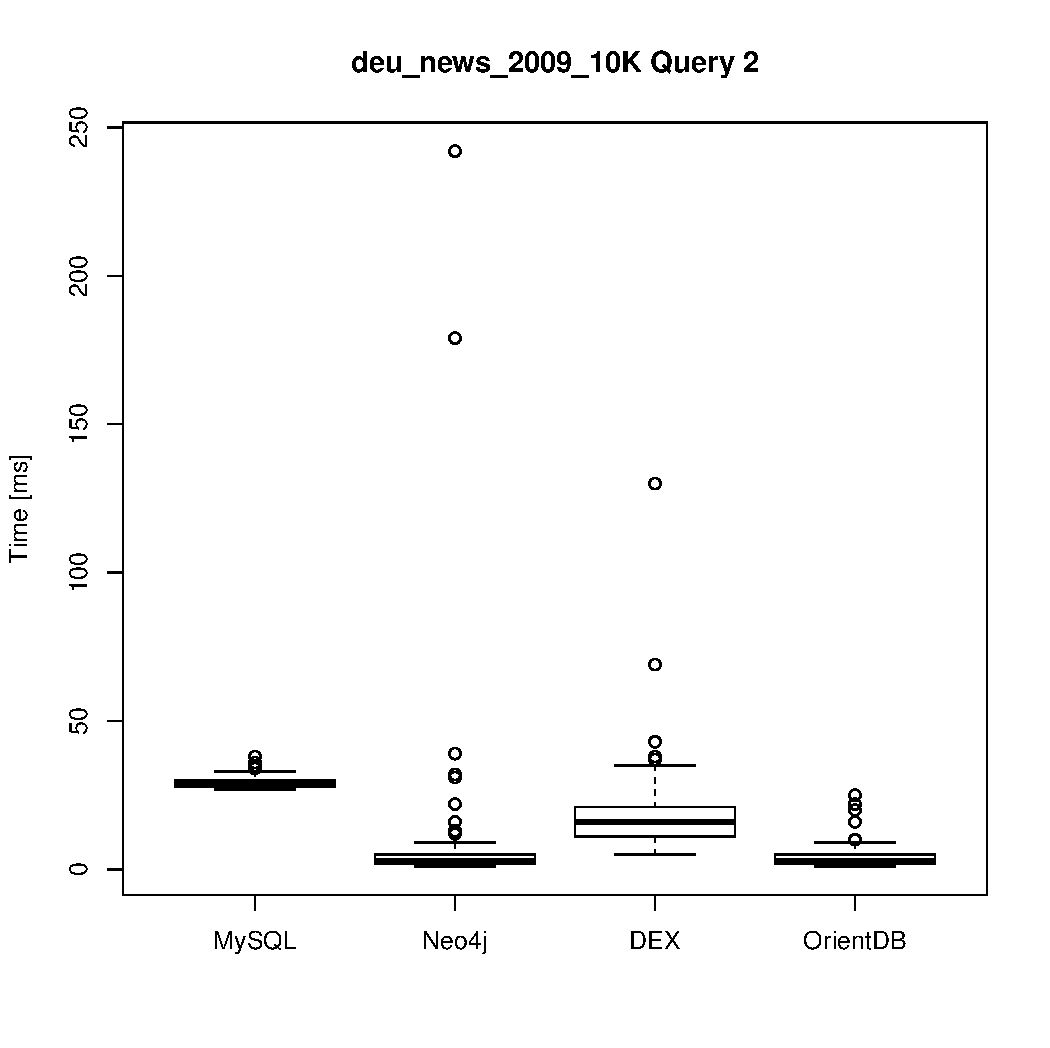
\includegraphics[width=7cm]{../results/cold caches/images/10K_query2_boxplot}
			\label{fig:10K_query2_boxplot}
		\end{minipage}
		\hfill
		\begin{minipage}[hbt]{6.5cm}
			\centering
			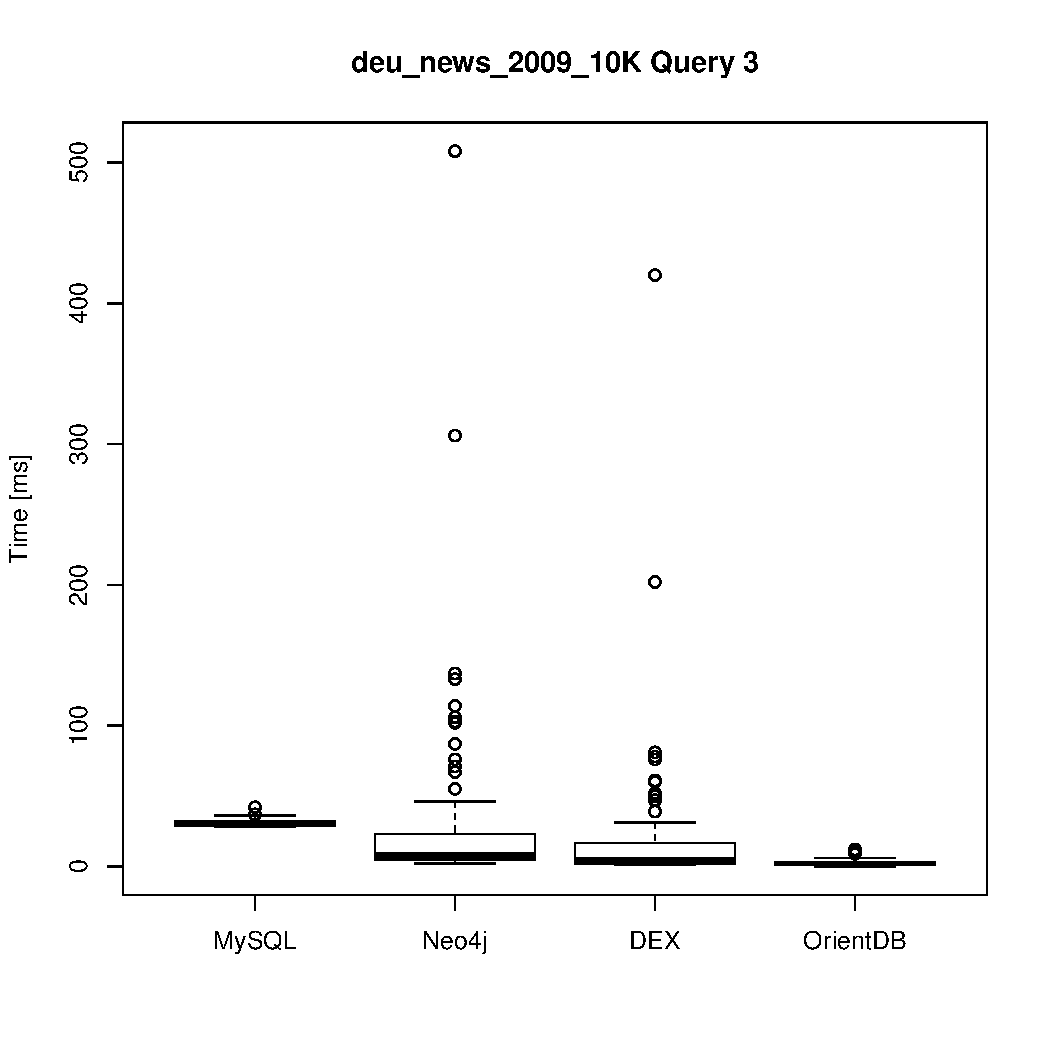
\includegraphics[width=7cm]{../results/cold caches/images/10K_query3_boxplot}
			\label{fig:10K_query3_boxplot}
		\end{minipage}
		
		\begin{minipage}[hbt]{6.5cm}
			\centering
			\includegraphics[width=7cm]{../results/cold caches/images/100K_query1_boxplot}
			\label{fig:100K_query1_boxplot}
		\end{minipage}
		\hfill
		\begin{minipage}[hbt]{6.5cm}
			\centering
			\includegraphics[width=7cm]{../results/cold caches/images/100K_query2_boxplot}
			\label{fig:100K_query2_boxplot}
		\end{minipage}
		\hfill
		\begin{minipage}[hbt]{6.5cm}
			\centering
			\includegraphics[width=7cm]{../results/cold caches/images/100K_query3_boxplot}
			\label{fig:100K_query3_boxplot}
		\end{minipage}
	\end{figure}
\end{landscape} 

\begin{landscape} 
	\newpage
	\thispagestyle{empty}
	
	\begin{figure}[ht]
		\begin{minipage}[hbt]{6.5cm}
			\centering
			\includegraphics[width=7cm]{../results/cold caches/images/1M_query1_boxplot}
			\label{fig:1M_query1_boxplot}
		\end{minipage}
		\hfill
		\begin{minipage}[hbt]{6.5cm}
			\centering
			\includegraphics[width=7cm]{../results/cold caches/images/1M_query2_boxplot}
			\label{fig:1M_query2_boxplot}
		\end{minipage}
		\hfill
		\begin{minipage}[hbt]{6.5cm}
			\centering
			\includegraphics[width=7cm]{../results/cold caches/images/1M_query3_boxplot}
			\label{fig:1M_query3_boxplot}
		\end{minipage}
		
		\begin{minipage}[hbt]{6.5cm}
			\centering
			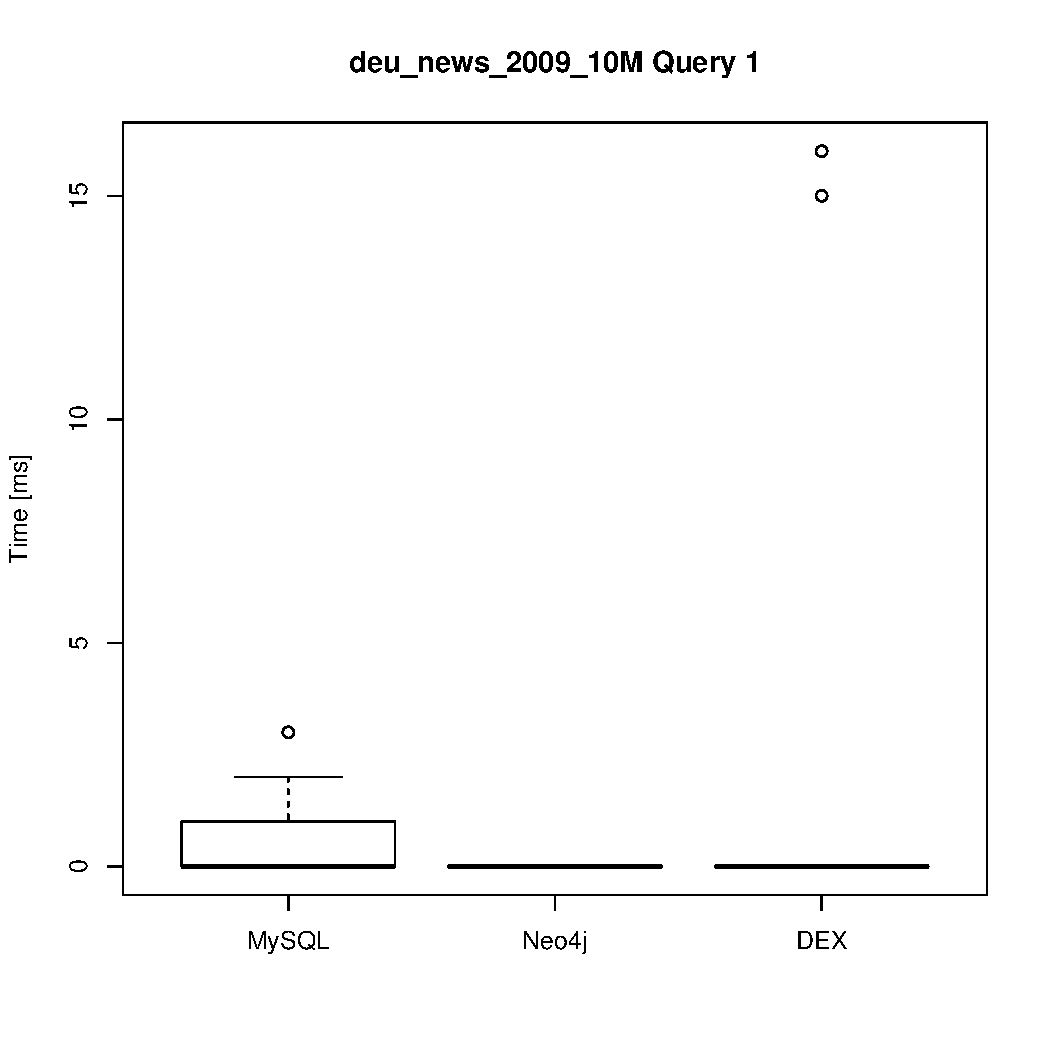
\includegraphics[width=7cm]{../results/cold caches/images/10M_query1_boxplot}
			\label{fig:10M_query1_boxplot}
		\end{minipage}
		\hfill
		\begin{minipage}[hbt]{6.5cm}
			\centering
			\includegraphics[width=7cm]{../results/cold caches/images/10M_query2_boxplot}
			\label{fig:10M_query2_boxplot}
		\end{minipage}
		\hfill
		\begin{minipage}[hbt]{6.5cm}
			\centering
			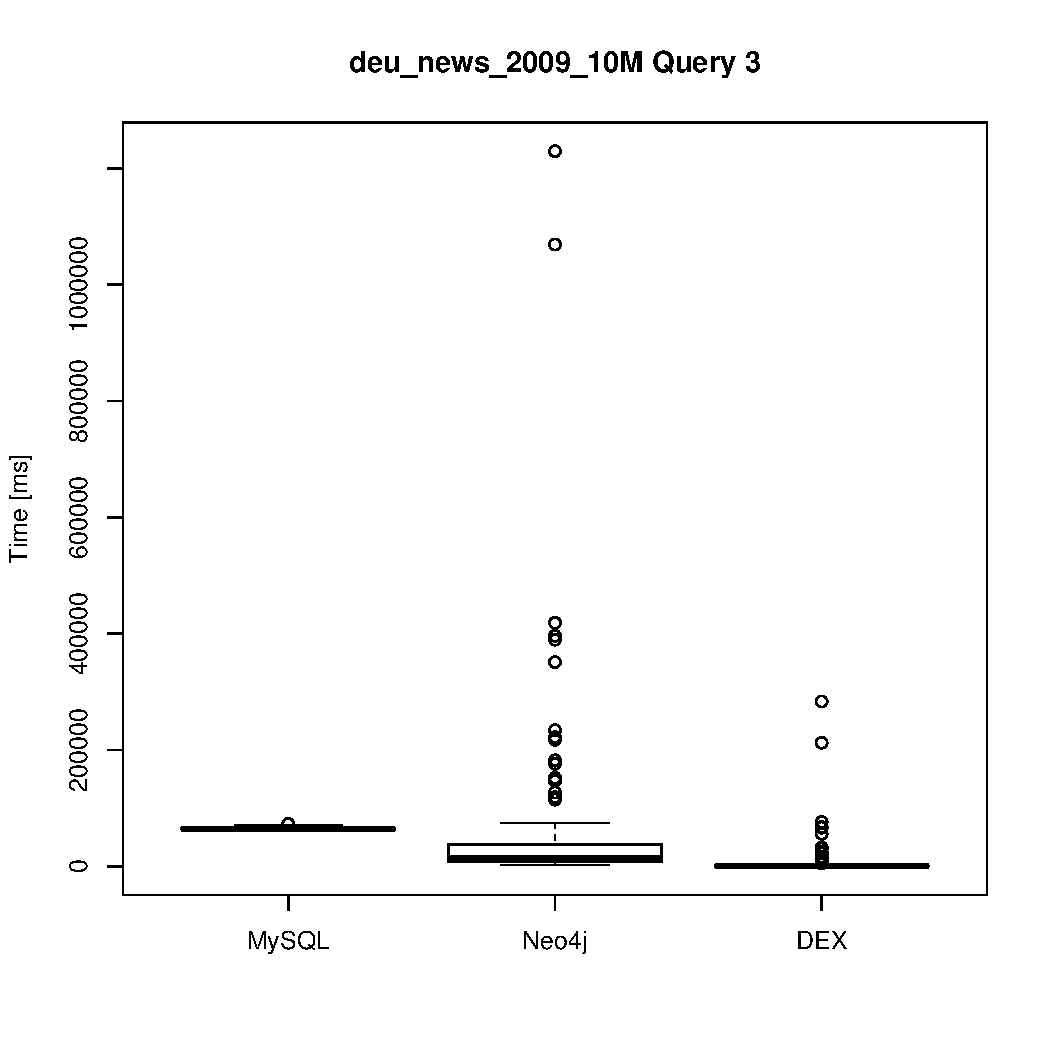
\includegraphics[width=7cm]{../results/cold caches/images/10M_query3_boxplot}
			\label{fig:10M_query3_boxplot}
		\end{minipage}
	\end{figure}
\end{landscape}

\begin{landscape} 
	\newpage
	\thispagestyle{empty}
	
	\begin{figure}[ht]
		\begin{minipage}[hbt]{6.5cm}
			\centering
			\includegraphics[width=7cm]{../results/cold caches/images/10K_query1_perf}
			\label{fig:10K_query1_perf}
		\end{minipage}
		\hfill
		\begin{minipage}[hbt]{6.5cm}
			\centering
			\includegraphics[width=7cm]{../results/cold caches/images/10K_query2_perf}
			\label{fig:10K_query2_perf}
		\end{minipage}
		\hfill
		\begin{minipage}[hbt]{6.5cm}
			\centering
			\includegraphics[width=7cm]{../results/cold caches/images/10K_query3_perf}
			\label{fig:10K_query3_perf}
		\end{minipage}
		
		\begin{minipage}[hbt]{6.5cm}
			\centering
			\includegraphics[width=7cm]{../results/cold caches/images/100K_query1_perf}
			\label{fig:100K_query1_perf}
		\end{minipage}
		\hfill
		\begin{minipage}[hbt]{6.5cm}
			\centering
			\includegraphics[width=7cm]{../results/cold caches/images/100K_query2_perf}
			\label{fig:100K_query2_perf}
		\end{minipage}
		\hfill
		\begin{minipage}[hbt]{6.5cm}
			\centering
			\includegraphics[width=7cm]{../results/cold caches/images/100K_query3_perf}
			\label{fig:100K_query3_perf}
		\end{minipage}
	\end{figure}
\end{landscape} 

\begin{landscape} 
	\newpage
	\thispagestyle{empty}
	
	\begin{figure}[ht]
		\begin{minipage}[hbt]{6.5cm}
			\centering
			\includegraphics[width=7cm]{../results/cold caches/images/1M_query1_perf}
			\label{fig:1M_query1_perf}
		\end{minipage}
		\hfill
		\begin{minipage}[hbt]{6.5cm}
			\centering
			\includegraphics[width=7cm]{../results/cold caches/images/1M_query2_perf}
			\label{fig:1M_query2_perf}
		\end{minipage}
		\hfill
		\begin{minipage}[hbt]{6.5cm}
			\centering
			\includegraphics[width=7cm]{../results/cold caches/images/1M_query3_perf}
			\label{fig:1M_query3_perf}
		\end{minipage}
		
		\begin{minipage}[hbt]{6.5cm}
			\centering
			\includegraphics[width=7cm]{../results/cold caches/images/10M_query1_perf}
			\label{fig:10M_query1_perf}
		\end{minipage}
		\hfill
		\begin{minipage}[hbt]{6.5cm}
			\centering
			\includegraphics[width=7cm]{../results/cold caches/images/10M_query2_perf}
			\label{fig:10M_query2_perf}
		\end{minipage}
		\hfill
		\begin{minipage}[hbt]{6.5cm}
			\centering
			\includegraphics[width=7cm]{../results/cold caches/images/10M_query3_perf}
			\label{fig:10M_query3_perf}
		\end{minipage}
	\end{figure}
\end{landscape}

\end{appendix}
\end{document}